\chapter{Proposed Solution}
\label{proposed_solution}

The aim of this chapter is to explain in detail the steps followed to conduct the experiment first introduced in section \ref{}.

As explained in section \ref{sec:previous_work}, the suppression of anger can derivate in the development on a more extremist and sarcastic personality. To recognize repressed anger from text messages, this research has based on the hypothesis that repressed anger messages contain both anger and ironic features and thus, focus on the detection of these features independently on Twitter documents.

Many research have been done to detect theses to aspects, in general, we could say that the most explored approach used for emotion classification and irony detection are based on \acrshort{svm} learning algorithm. However, recently introduced technology has been gaining popularity among researchers: \acrshort{dl}. In fact, during the task four presented in the international workshop of evaluations of computational semantics, SemEval 2016, the organizers stated as follow:

\textit{``A general trend that emerges from SemEval-2016 Task 4 is that most teams who were ranked at the top in the various subtasks used \acrlong{dl}, including convolutional \acrshort{nn}, recurrent \acrshort{nn}, and (general purpose or task-specific) word embeddings. In many cases, the use of these techniques allowed the teams using them to obtain good scores even without tuning their system to the specifics of the subtask at hand [...]. Conversely, several teams that have indeed tunned their system to the specifics of the subtask at hand, but have not used \acrlong{dl} techniques, have performed less satisfactorily. This is a further confirmation of the power of \acrlong{dl} techniques for tweet sentiment analysis''} \cite{nakov2016semeval}.

\acrshort{dl} has caused a great impact on SemEval and recent researches and therefore, based on these statements the decision to implement a system that make used of this technique was made.

Since \acrshort{dl} is a class of \acrshort{ml}, the procedure developed in the proposed solution (see figure \ref{fig:solution_procedure}) follows the steps of a classical \acrlong{ml} approach (section \ref{subsubsec:techniques_machine_learning}): data collection, pre-processing, learning process, prediction and evaluation. In the following sections a general perspective of the proposed solution will introduced followed up by an explanation of the four steps in detail, while evaluation results will be presented of the following chapter.

\begin{figure}[!htp]
  \center
  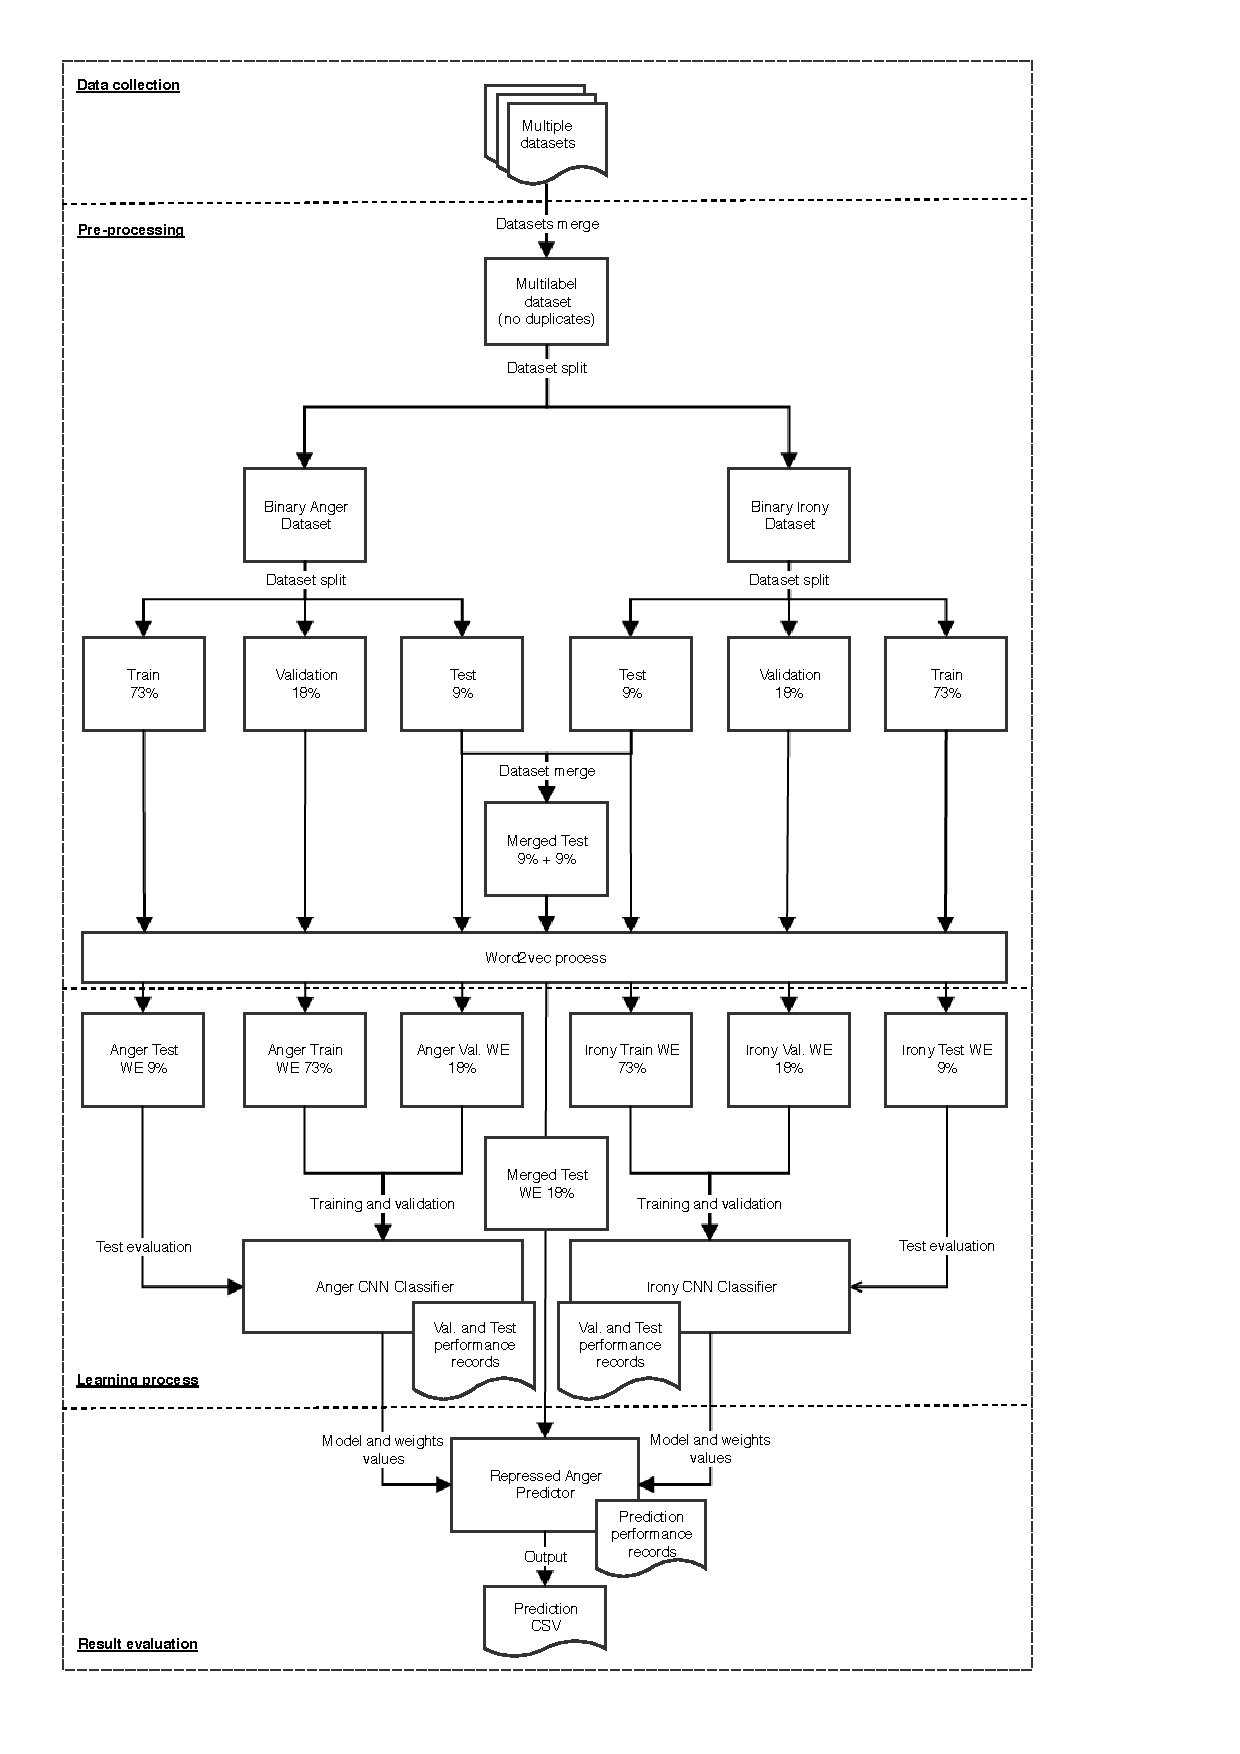
\includegraphics[width=0.93\textwidth]{figures/flow}
  \caption{Proposed solution procedure.}
  \label{fig:solution_procedure}
\end{figure}

\section{Data Collection}

The objective of subtask is to gather already annotated tweets that contains emotions, specially anger, and irony. During this step, multiple research paper that would provide public available dataset or would provide the methodology on how to build one were analyzed, such as the explained in \cite{hasan2014emotex} and \cite{sulis2016figurative}. In the following paragraphs describe the public datasets gathered and created for this project.

\subsection{Wang's SMILE Twitter emotion dataset}

At first, only Wang et al.'s SMILE Twitter emotion dataset was found, containing a total of 3,085 tweets classified as: anger, disgust, happy, no-code, not-relevant, sad and surprise \cite{wang2016smile}. By simply taking into account the number of tweets offered in this dataset as small, and probably not enough, to perform \acrshort{dl} based classification. Figure \ref{fig:smile_dataset_distribution} shows the distribution of tweets related to each annotated class. By analyzing the number of tweets related to anger the amount of tweets are reduced to 57. Moreover, the tweets labeled as not-relevant and no-code, classes that contains no value to the purpose of the research, represents around 58\% of the whole dataset. However, even if not being enough, the remaining 42\% would be stored to posteriorly merged to other datasets.

\begin{figure}[!htp]
  \center
  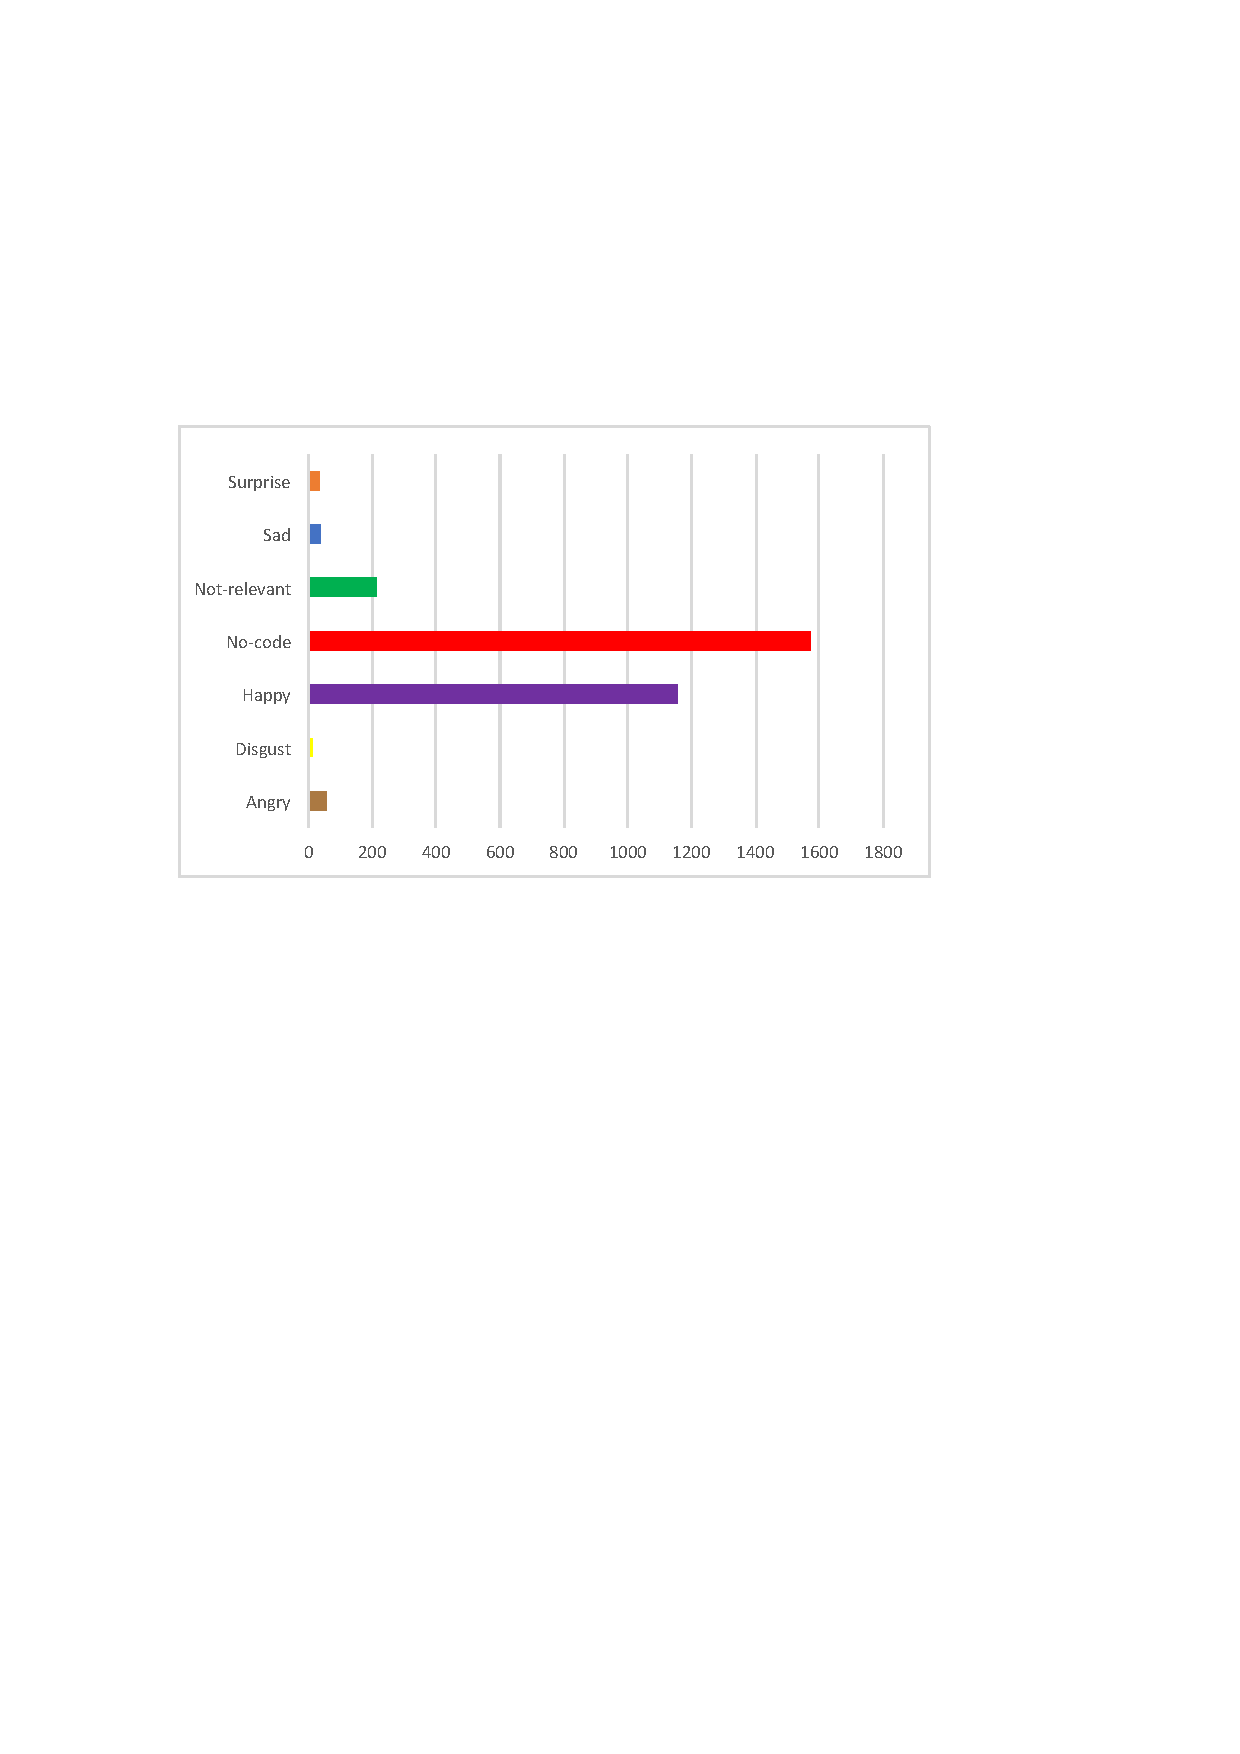
\includegraphics[width=0.5\textwidth]{figures/SMILE_dataset_distribution}
  \caption{Wang's SMILE Twitter emotion dataset distribution.}
  \label{fig:smile_dataset_distribution}
\end{figure}

\subsection{CrowdFlower's Data for Everyone, Sentiment Analysis: Emotion in Text dataset}

CrowdFlower, an \acrshort{hit} web solution, offers publicly available datasets under its ``Data for Everyone'' section, where an annotated emotion dataset for sentiment analysis can be downloaded for research purposes. The dataset is composed from tweets classified as the following 13 classes: anger, boredom, empty, enthusiasm, fun, happiness, hate, love, neutral, relief, sadness, surprise and worry \cite{CrowdFlowerDfE}. Figure \ref{fig:crowdflower_dataset_distribution} shows the number of tweets per annotated class, being anger and hate the most relevant for the purpose of this project representing around 3\% of the dataset.

\begin{figure}[!htp]
  \center
  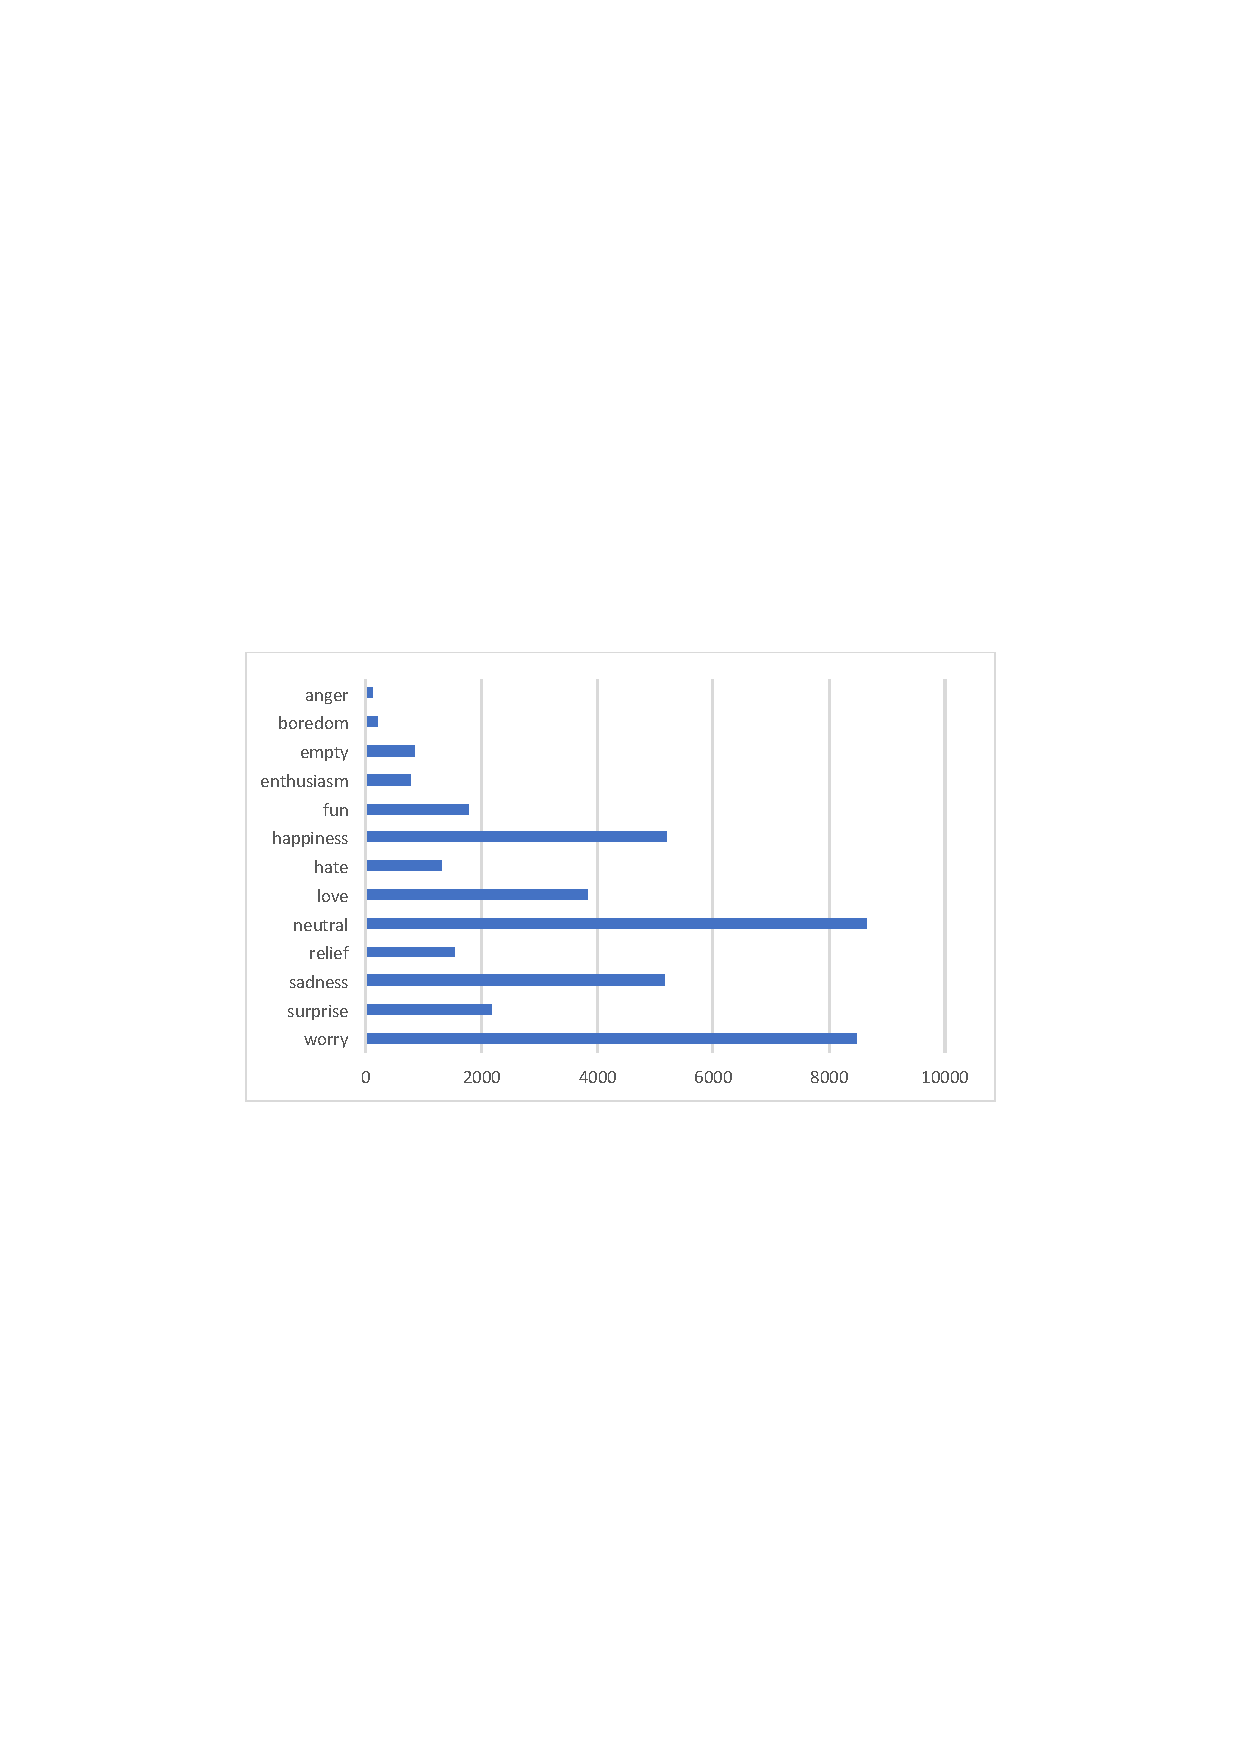
\includegraphics[width=0.6\textwidth]{figures/crowd_flower_dataset_distribution}
  \caption{CrowdFlower's Data for Everyone, Sentiment Analysis: Emotion in Text dataset distribution.}
  \label{fig:crowdflower_dataset_distribution}
\end{figure}

\FloatBarrier

\subsection{Wang 2012, Harnessing Twitter ``big data'' dataset}

In 2012 Wang et al. created a publicly available dataset from Twitter messages to analyze emotions. The dataset is composed from tweets classified in 7 categories as anger, fear, joy, love, sadness, surprise and thankfulness \cite{wang2012harnessing}. However, due to the term of service of Twitter, \textit{``If you provide Content to third parties, including downloadable datasets of Content or an API that returns Content, you will only distribute or allow download of Tweet IDs and/or User IDs''} \cite{twitterTOS} and thus, this dataset does not contain the proper tweet message, but a identifier number instead. To download the content of the tweet an Twitter Python \acrshort{api} known as Tweepy \cite{Tweepy} was used over the dataset's ``test'' and ``train\_2\_1'' files. Although, since the originally the tweets were collected on 2011 to build the dataset, nowadays not all the tweets are available, as some users have removed their account or change their privacy settings. Figure \ref{fig:wang_2012_dataset_distribution} shows the number of tweets that were able to collect per class.

\begin{figure}[!htp]
  \center
  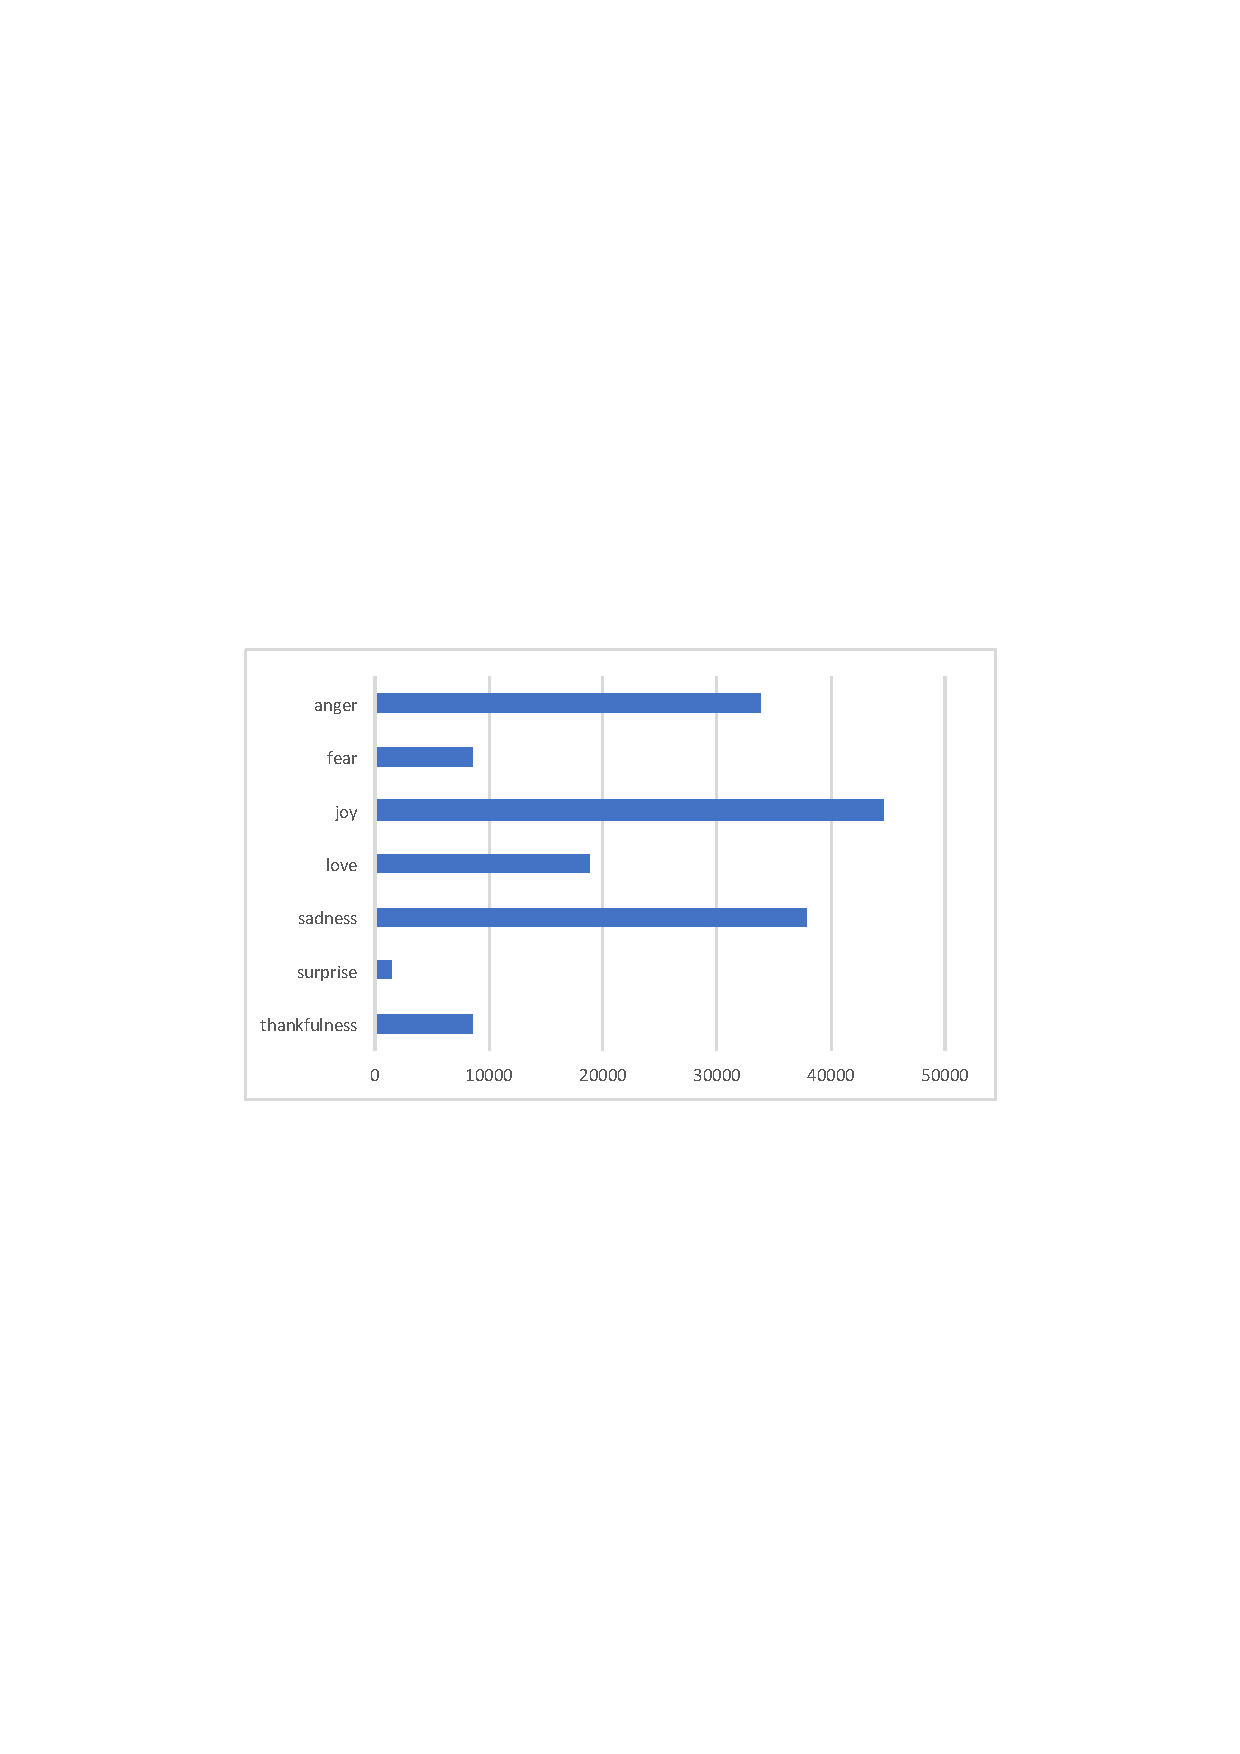
\includegraphics[width=0.6\textwidth]{figures/wang_2012_dataset_distribution}
  \caption{Wang 2012's test and train\_2\_1 datasets merged distribution.}
  \label{fig:wang_2012_dataset_distribution}
\end{figure}

\subsection{Harvesting Irony dataset}

To collect tweets related to irony, as no publicly available dataset was found on a reasonable time, it was decided to harvest automatically annotated tweets directly. To do so, Twitter archiver \cite{twitterArchiver}, an extension of Google Sheets, was used. It enables to automatically download tweets based on features such as keywords, hashtags, language, among others. By using this tool a total of 36,274 English tweets that contained hashtags such as \#irony, \#ironic, \#sarcasm or \#sarcastic where downloaded from December 12th 2016 to January 25th 2017.

\section{Pre-processing}

After having collected enough data to prevent \acrshort{dl} overfitting issue, the next step is to pre-process the datasets, to eliminate non English tweets, possible duplicates, hashtags, user references, \acrshortpl{url}, correct spell mistakes, filter undesired classes, among others.

\begin{figure}[!htp]
  \center
  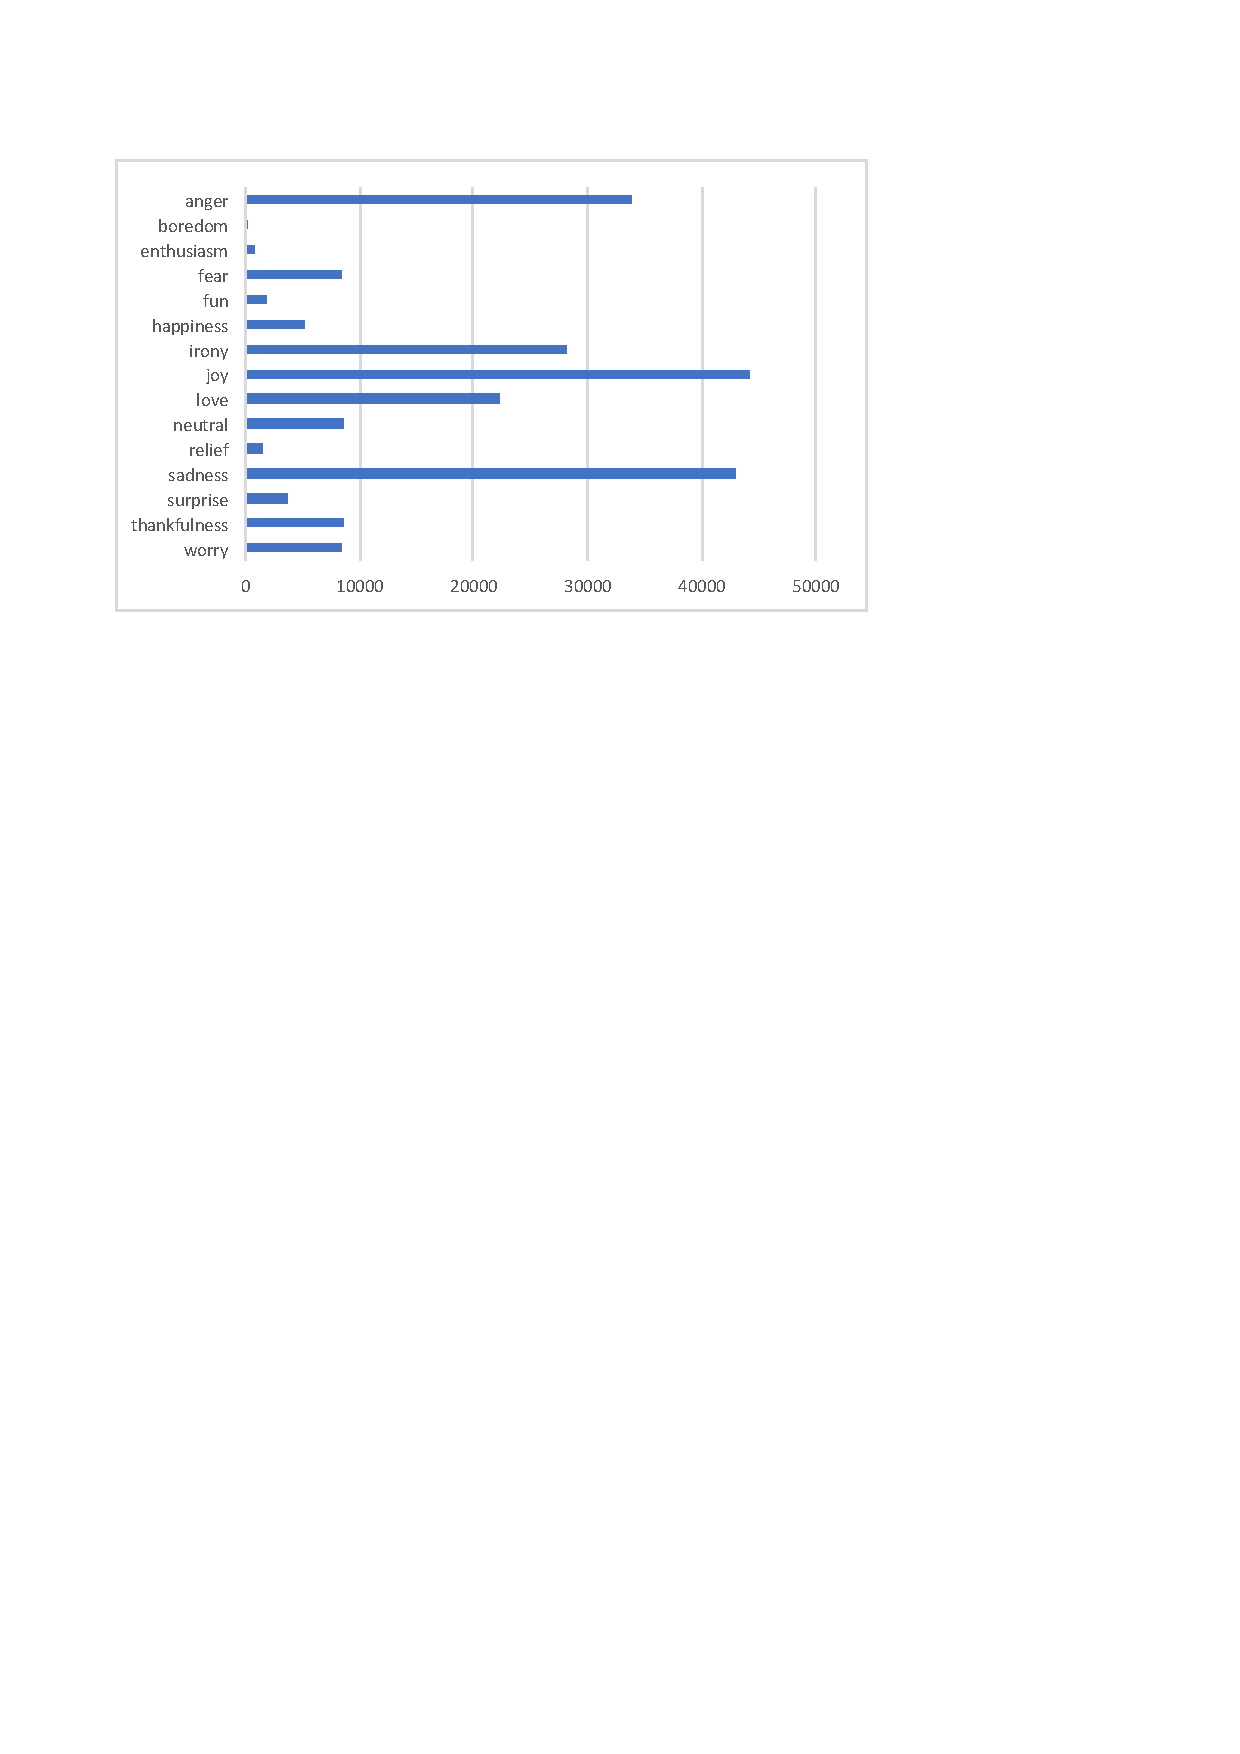
\includegraphics[width=0.7\textwidth]{figures/merged_multilabel_dataset_distribution}
  \caption{Merged multi label dataset distribution.}
  \label{fig:merged_multilabel_dataset_distribution}
\end{figure}

The first step of pre-processing was to delete all duplicates. To do so, all the data was merged into a single dataset file from which all the tweets that contain the same identification number (real duplicate instances) or tweet sharing same text message (possible re-tweets) were deleted. After delete non English tweets and filter ambiguous target labels from the file, the final dataset was composed by a total of 218,619 tweets grouped into 15 categories classified as: anger, boredom, fear, fun, happiness, irony, joy, love, neutral, relief, sadness, surprise, thankfulness and worry. Figure \ref{fig:merged_multilabel_dataset_distribution} shows the distribution of each label target.

Because anger and irony are analyzed independently in this project, to isolate each classifier two datasets were built: binary anger dataset and binary irony dataset. As their name suggest, each dataset is composed by tweets grouped into two classes, the pairs ``anger'', ``no\_anger'' and ``irony'', ``no\_irony'' label targets. To prevent the learning process to be biased into one class or the other, the data was under-sampled to match the number of instances appearances of the anger and irony tweets in the previously merged multi-label dataset to created balanced datasets. Thus, binary anger dataset is composed by a total of 67,748 tweets, 33,874 for ``anger'' annotated tweets and the same amount for ``no\_anger'' related tweets (see Figure \ref{fig:binary_anger_dataset_distribution}). Regarding to binary irony dataset, it is formed by 28,132 tweets for irony and the same amount for ``no\_irony'', making a total 56,264 tweets (see Figure \ref{fig:binary_irony_dataset_distribution}).

\begin{figure}[!htp]
  \center
  \begin{subfigure}[b]{0.5\textwidth}
    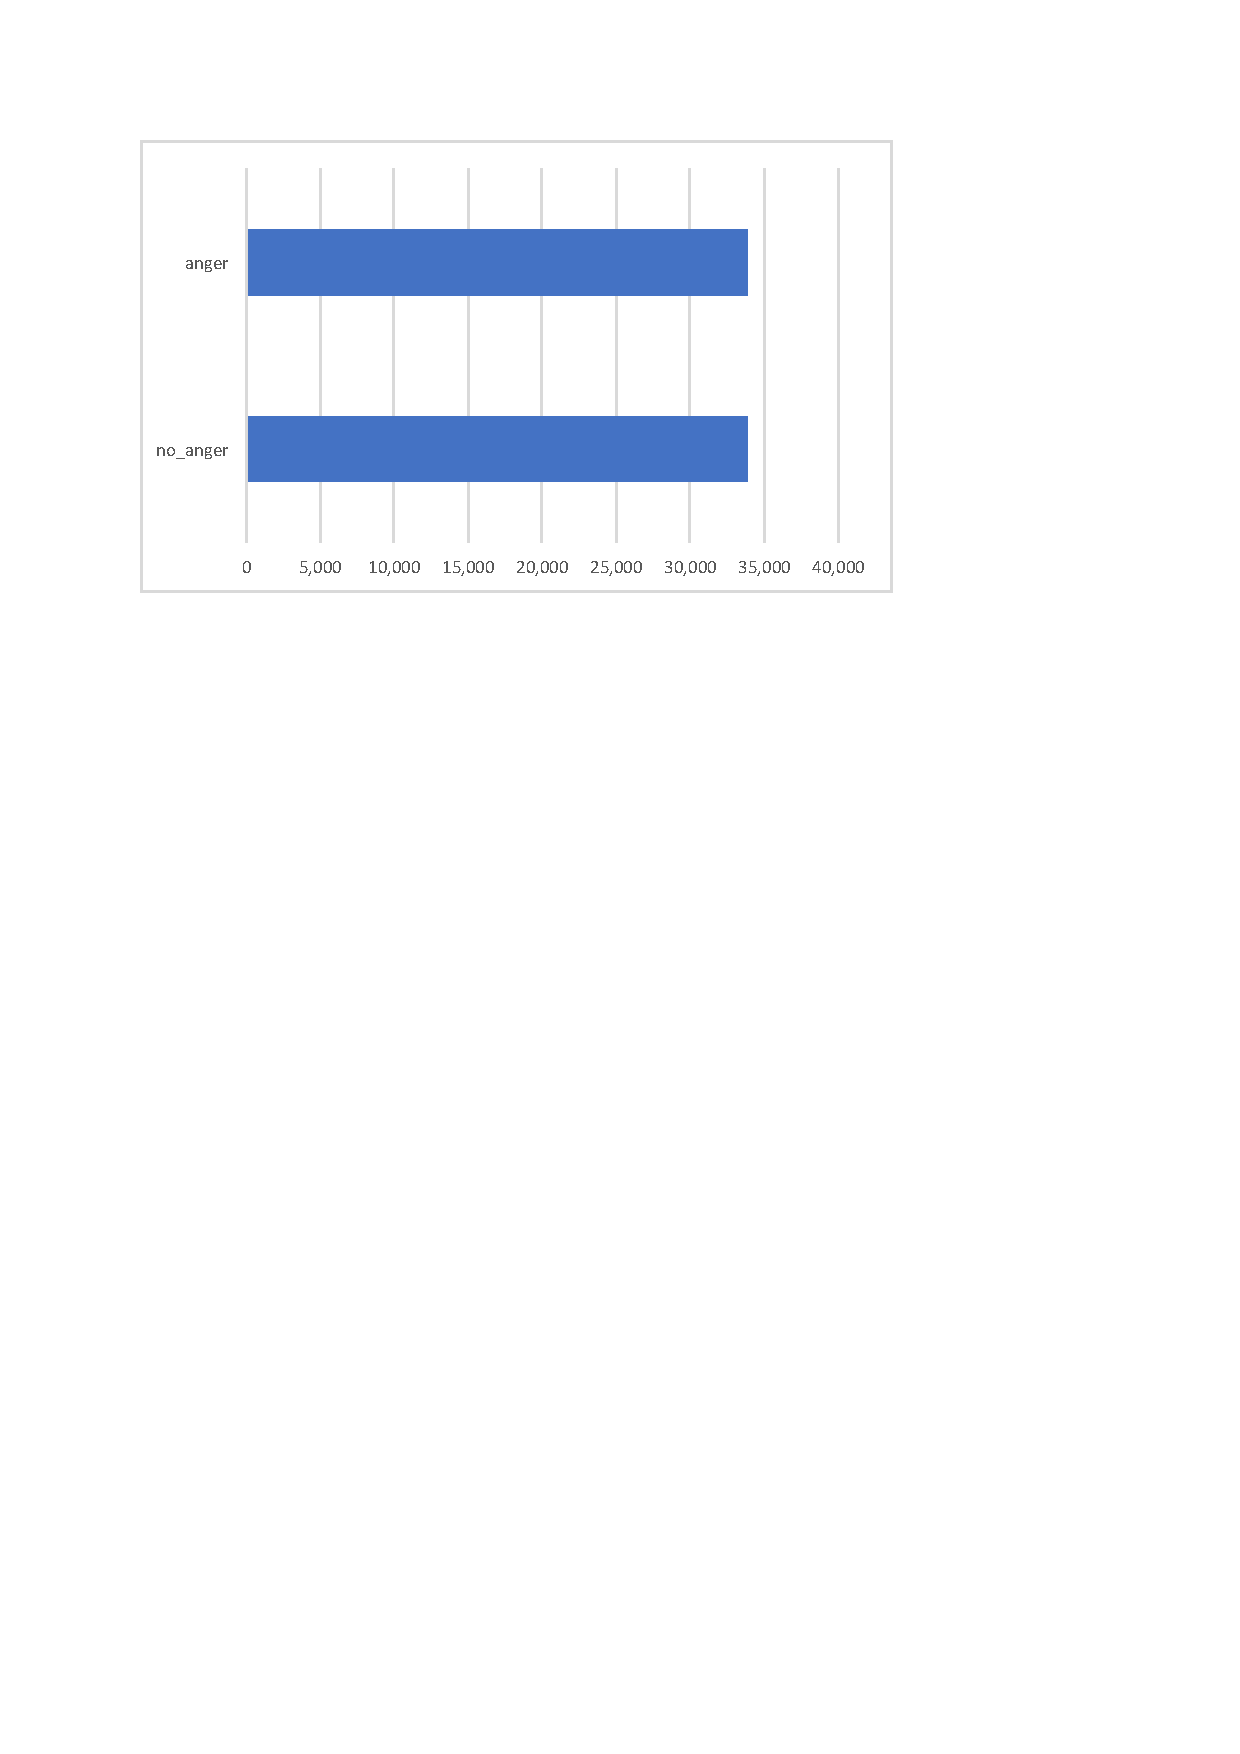
\includegraphics[width=\linewidth]{figures/binary_anger_dataset_distribution}
    \caption{Balanced binary anger dataset}
    \label{fig:binary_anger_dataset_distribution}
  \end{subfigure}%
  \begin{subfigure}[b]{0.5\textwidth}
    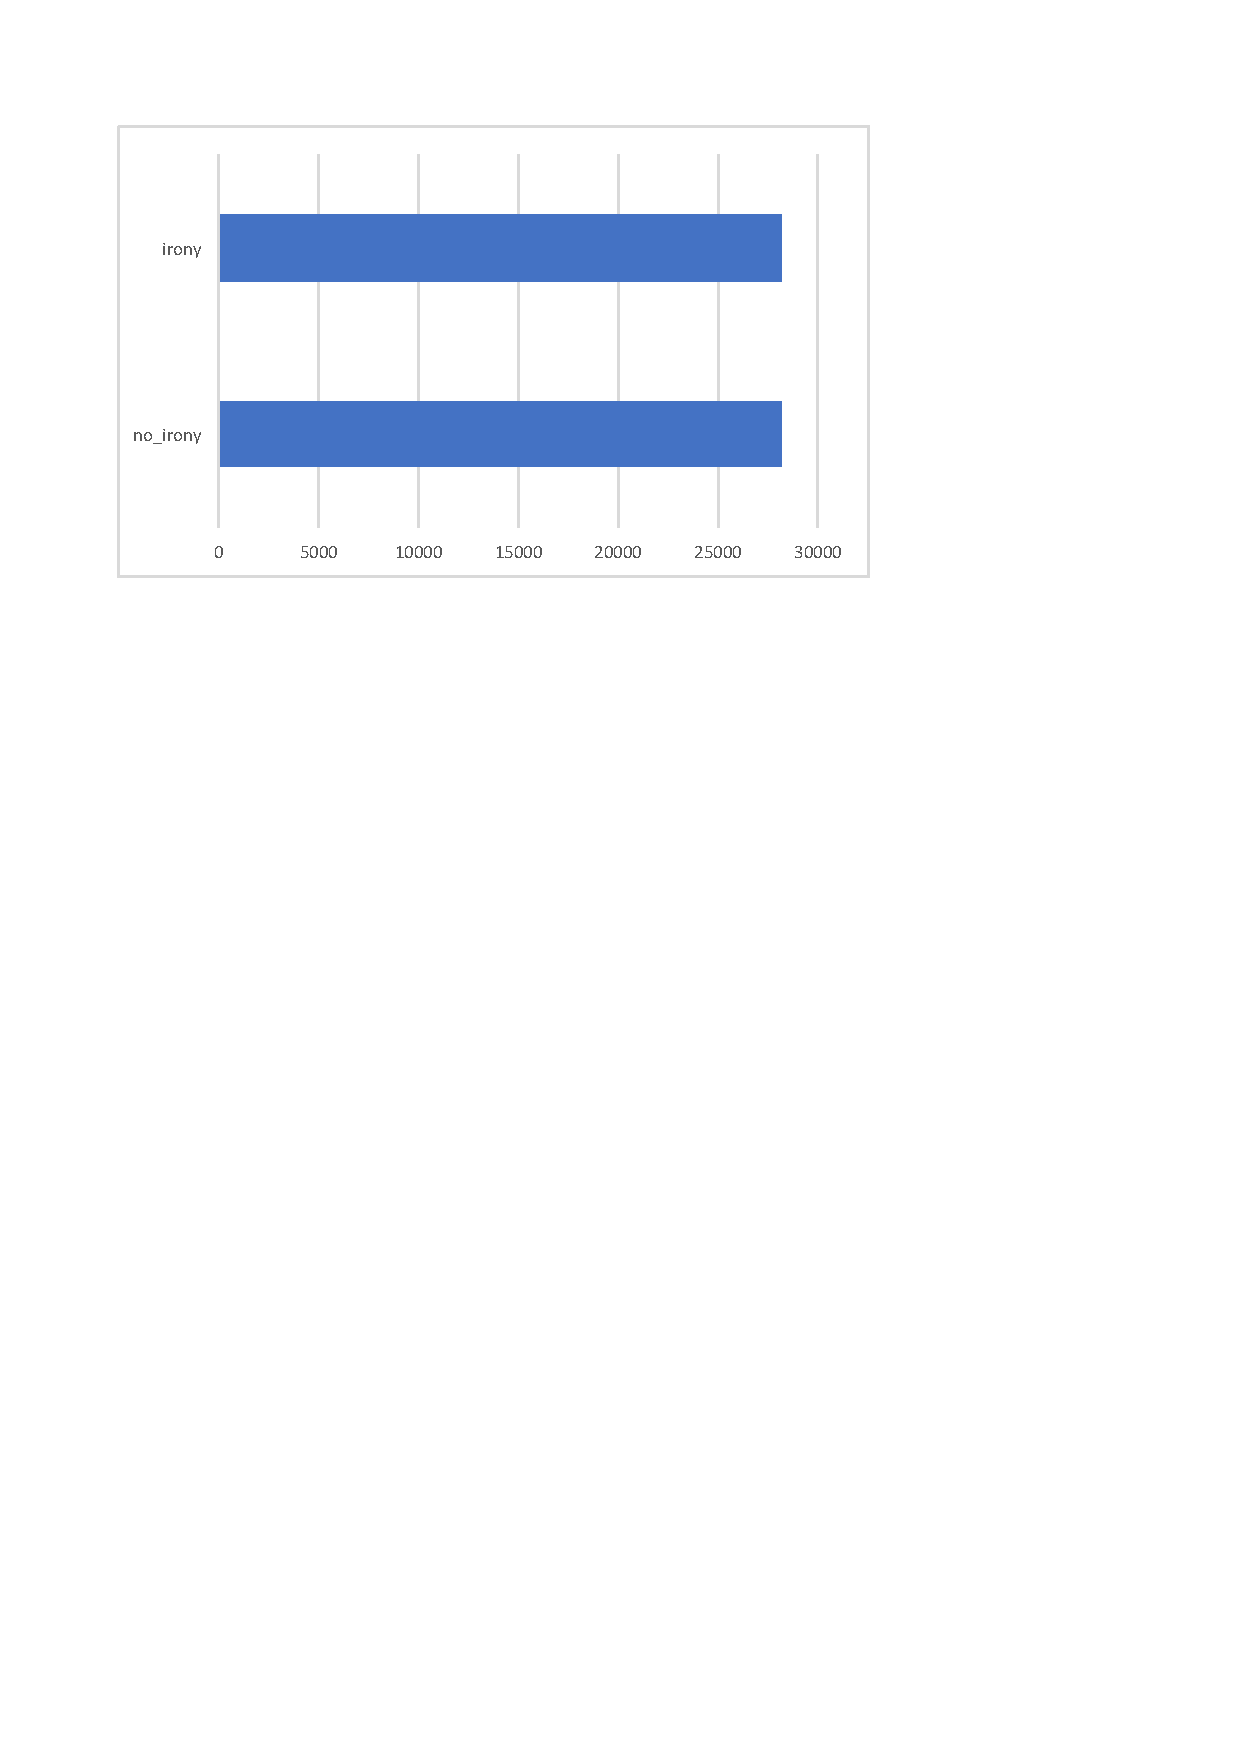
\includegraphics[width=\linewidth]{figures/binary_irony_dataset_distribution}
    \caption{Balanced binary irony dataset}
    \label{fig:binary_irony_dataset_distribution}
  \end{subfigure}%
  \caption{Dataset under-sampling}\label{fig:dataset_undersampling}
\end{figure}

To prepare the datasets for the posterior learning process, each dataset is divided into train, validation and test subsamples. Normally the division would be split into 70\% training, 15\% validation and 15\% test, however, as in the last prediction phase the test sample is produced by merging both anger and irony test files, these percentages were changed to 73\%, 18\% and 9\% respectively, to make the merged test file size have nearly the same size as each dataset validation files. Once both dataset have been split and the final prediction file generated by merging both datasets' test files, all the resulting files enter the word2vec process to generate the word embeddings files that will later on serve as input for the \acrshort{cnn} learning process.

\begin{figure}[!htp]
  \center
  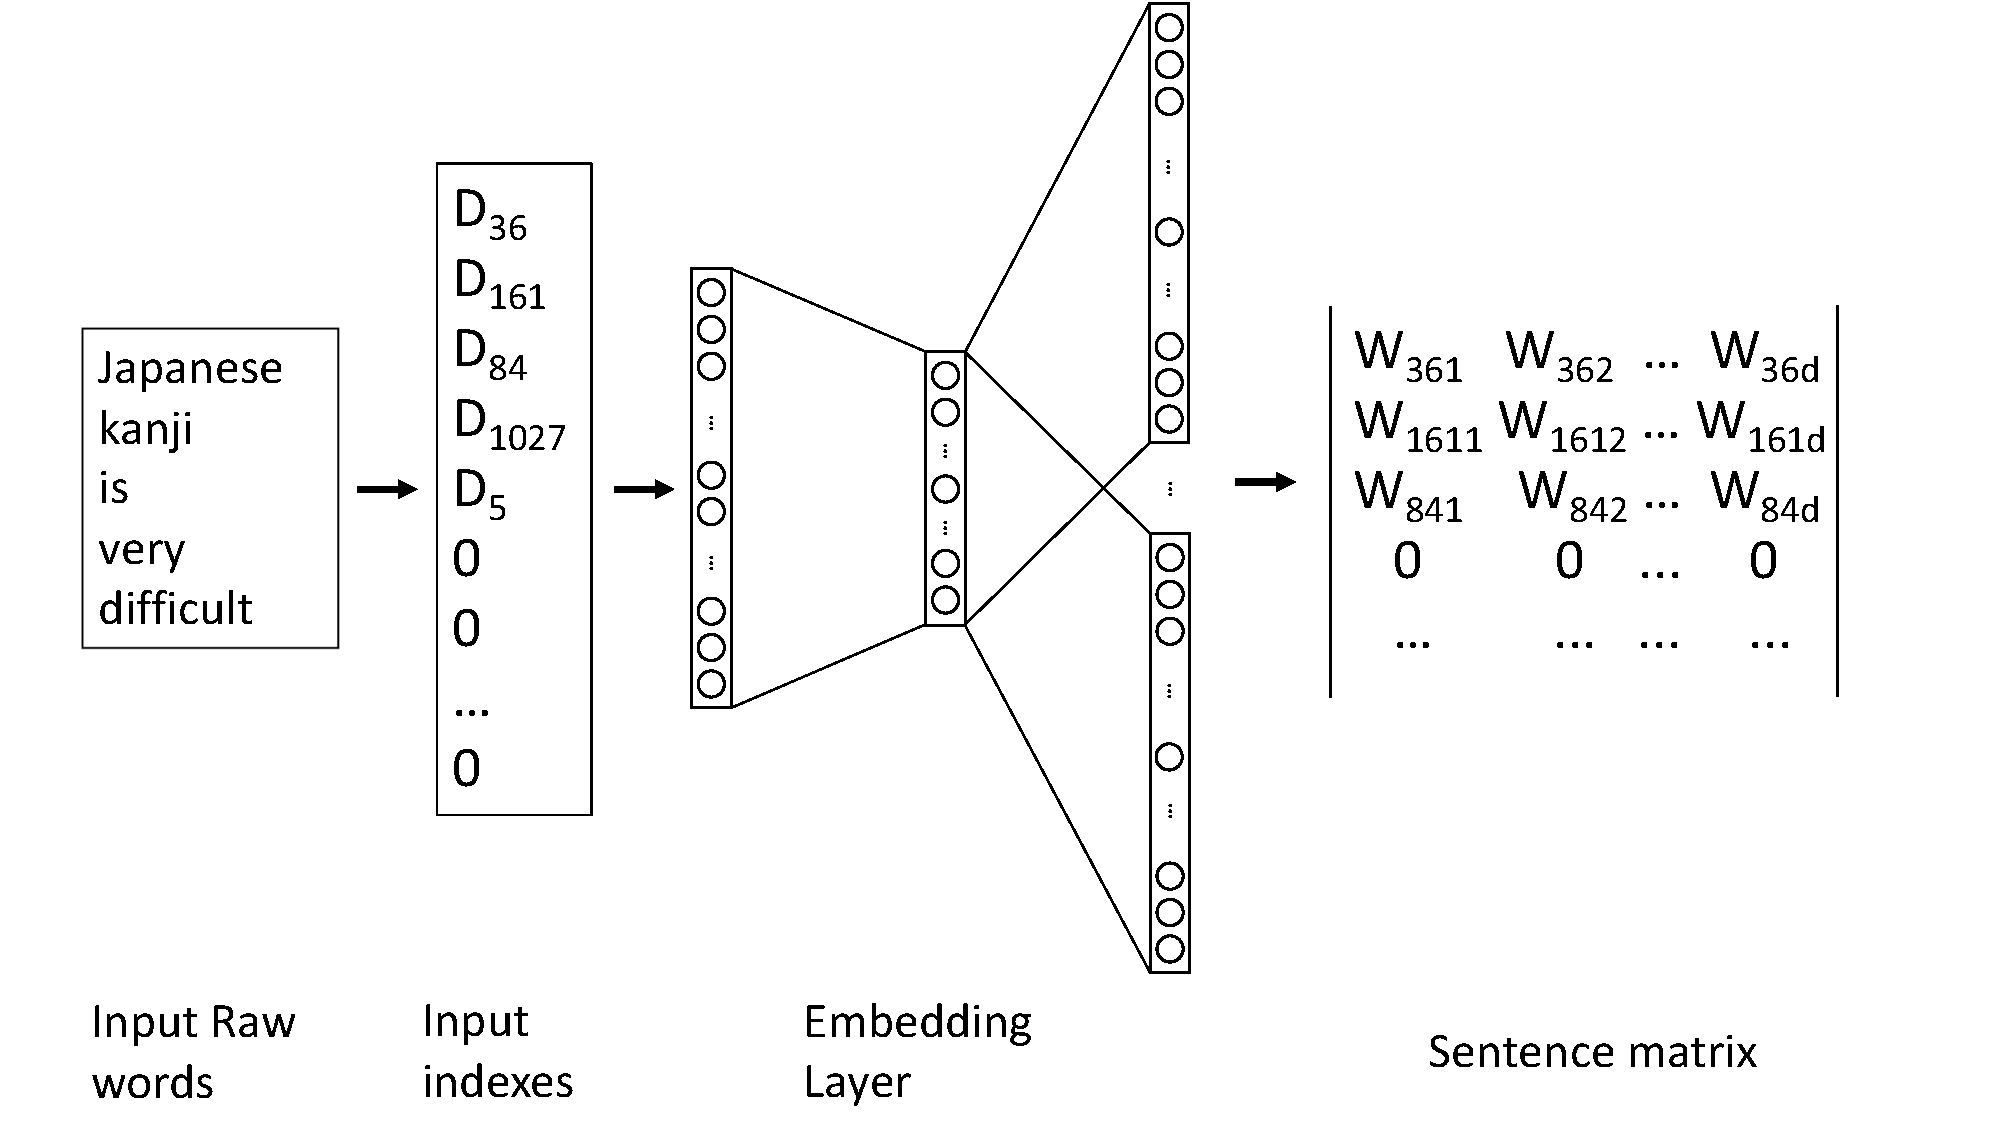
\includegraphics[width=0.85\textwidth]{figures/raw_text_word_vector_transformation}
  \caption{Raw word sentence to word vector matrix transformation.}
  \label{fig:raw_text_word_vector_transformation}
\end{figure}

During this process the pre-processing of the tweets that compose the corpus occurs and all the hashtags, user references, \acrshortpl{url} are replaced by identification tags such as TAG, MENTION and URL, stopwords are removed from the sentences and optionally all the remaining words are checked and replaced by using Peter Norvig's spell checker \cite{PeterNorvigSpell} with an own made language model generated from calculating the word appearance of 36,173 free English \acrshort{html} eBooks extracted by Kiwix harvester (2014) \cite{kiwix} Project Gutenberg \cite{projectGutenberg}, most used frequency words list obtained from TV programs and contemporary fiction books from Wiktionary \cite{WiktionaryFL}, film series from Opensubtitles extracted by Hermit Dave \cite{openSubtitlesFL} and \acrfull{bnc} \cite{bncFLAdamK}. Since the learning process requires to introduce a sequence of words of a fixed length, we decided the value based on the length of the phrase length of our corpus, and thus, calculated the maximum sentence length of both anger (29) and irony (28) datasets and select the maximum value (29) as the fixed sequence length for the model generation. All tweets sentences composing the corpus are transformed sequences of 29 indexes by using a dictionary $D$ that contains the mapping to indexes of millions of words. Then, by ploying a embedding layer, each of those indexes are converted into space vectors, which are initialized by using the Word2Vec algorithm \cite{mikolov2013efficient}. The combination all the space vectors that compose the original tweet sentence creates an output matrix $M\in\mathbb{R}^{29 \times d}$, where $d$ represents the length of the word embeddings (see figure \ref{fig:raw_text_word_vector_transformation}). As not all the input sentences contain 29 words, each matrix is padded with 0s until reaching the fixed sentence length. Finally, the list of generated matrices are stored for their later use on the learning and prediction processes.

\section{Learning process}

The learning solution proposed consist on a hybrid approach that combines the prediction output of two deep neural network classifiers. To design the architecture of each classifier, we followed the work of Kim \cite{kim2014convolutional}, which uses \acrshort{cnn} for sentence classification. The input of this architecture is an sequence of words, more precisely, the list of word embedding matrices generated on the previous word2vec process. Our model is fed with each matrix and performs convolution operations with multiple filters to learn from multiple features as stated in \cite{zhang2015sensitivity}. We have experimented using 200 filters of 3 sizes (3, 4 and 5) with a ReLU activation function. The functionality of these filters can be compared with how n-grams based classification work \cite{cavnar1994n}. Our model relies on what on n-grams would be considered as 3-grams, 4-grams and 5-grams. The n-grams are extracted from input matrix, in which each row represents a word from the tweet. Each filter combines a groups of 3, 4 or 5 rows obtaining all the possible n-grams from the sentence, generating as a result, a feature map. This map serve as the input of the next max-pooling layer. Its objective is to reduce the profile and bandwidth of the input matrix for computational purposes. Although multiple pooling strategies exist \cite{boureau2010theoretical}, the experiments performed in \cite{zhang2015sensitivity} shows that max-pooling strategy outperforms the rest and thus, selected this strategy to develop our model. It extracts only the feature with the highest value from the initial feature map. When all the features maps from each filter have been processed, the extracted features are then concatenated into a single feature vector to which a dropout layer of rate 0.5 is applied as a measure to prevent the model from over-fitting \cite{srivastava2014dropout}. The model ends with a final softmax layer that calculates the probability distribution over the output vector, representing the classification into the target labels. For training purpose, a categorical cross-entropy loss function has been used with Adam optimizer \cite{kingma2014adam}. The figure \ref{fig:designed_architecture} illustrates designed architecture using 2 filters instead of 200 for explanatory purposes.

\begin{figure}[!htp]
  \center
  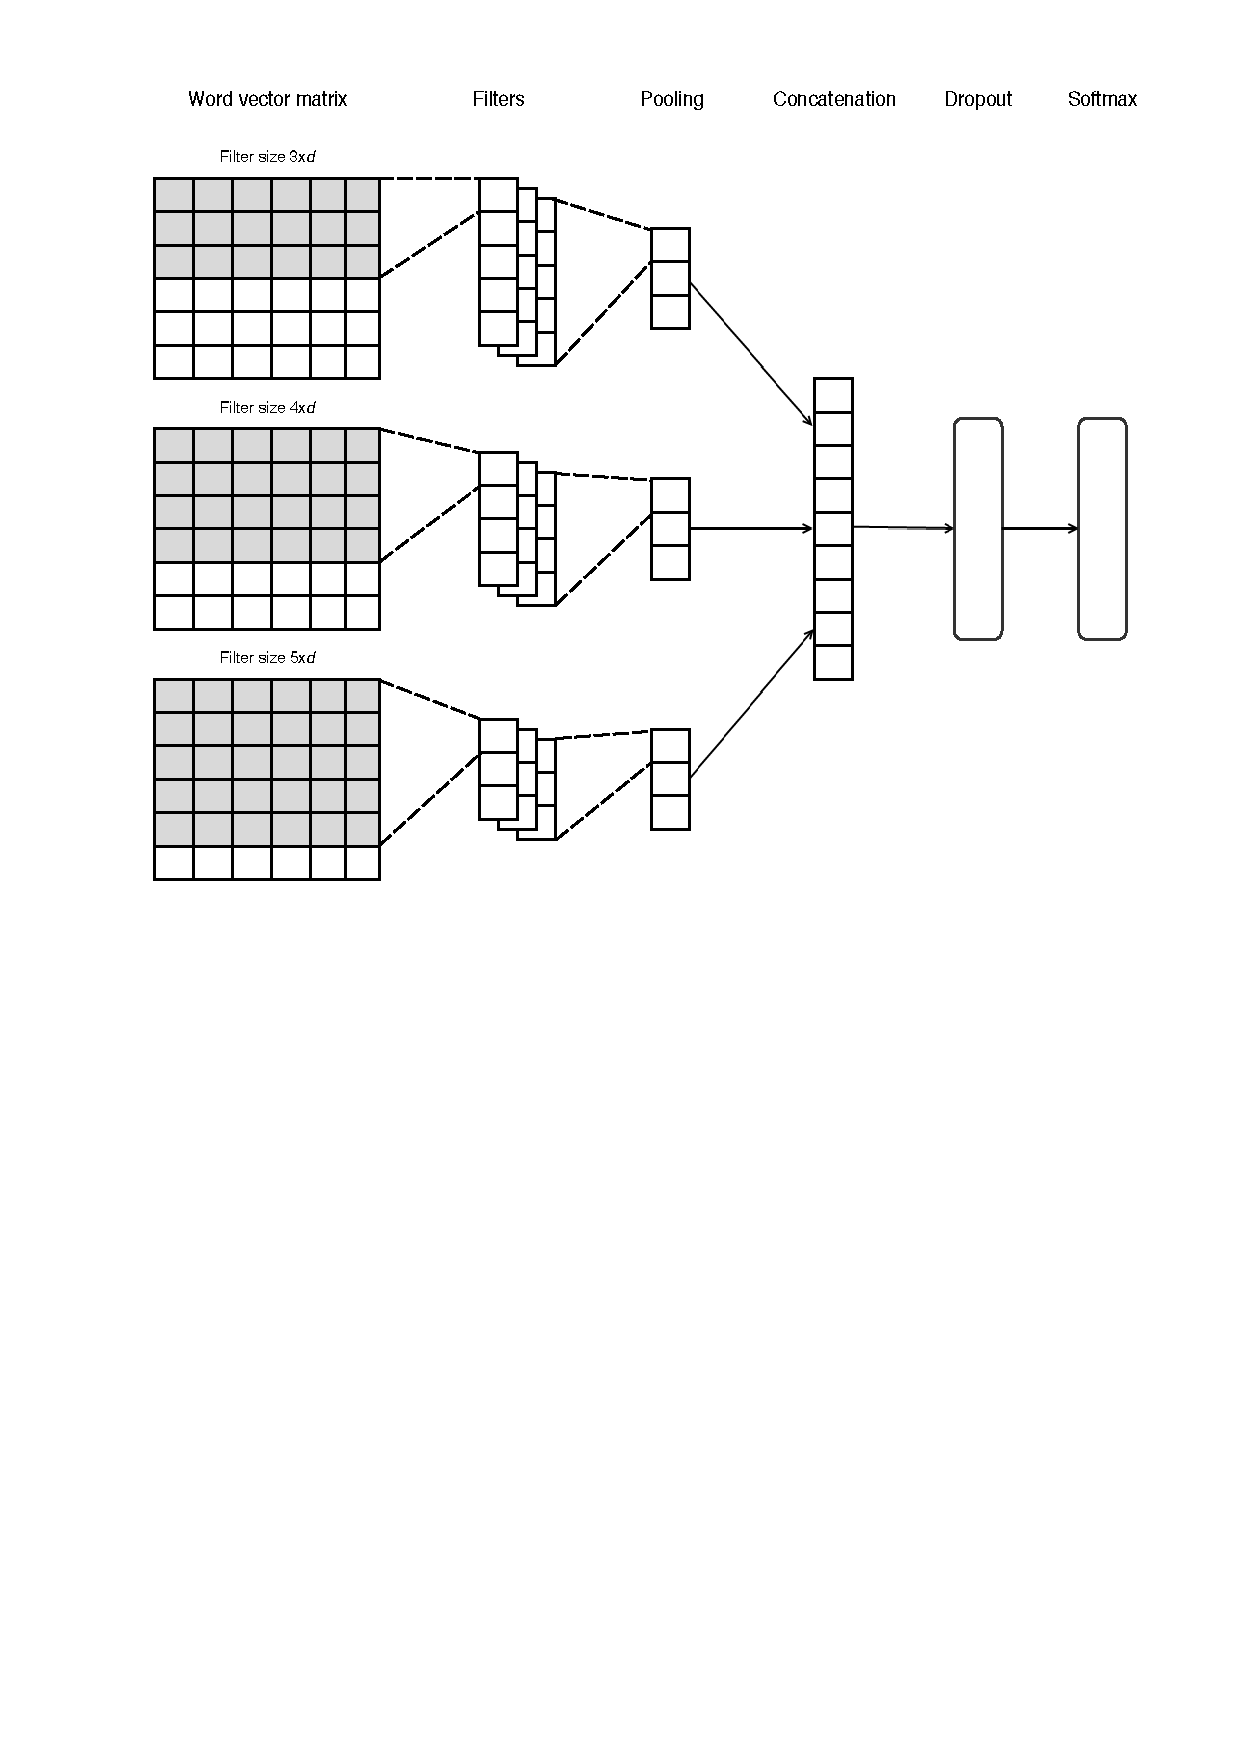
\includegraphics[width=0.81\textwidth]{figures/designed_architecture}
  \caption{Designed architecture.}
  \label{fig:designed_architecture}
\end{figure}

\section{Prediction}

Once both classifiers have been trained and validated with the corresponding word embeddings matrices files two files are generated per classifier: the model, which saves the architecture of the classifier, and the weights in which the classifier has obtained best result during the learning process. Having as a input file the combination of each classifier test sample, theses four files are used to load the anger and irony classifiers' parameters to perform the prediction of new data. Each classifier generates a binary class output prediction of a given tweet that need to be combined. Although the usage Ensemble Learning based on divide and conquer \cite{ensemble2009Polikar} approach was studied to merge classifiers, as each classifier works with its own set target labels independently this idea was discarded. Thus, the solution proposed, following the definition of repressed anger personality first presented in section \ref{sec:previous_work}, consists on merging the output of the classifiers generating four target labels according to the matrix presented in figure \ref{fig:merge_matrix}.

\begin{figure}[!htp]
  \center
  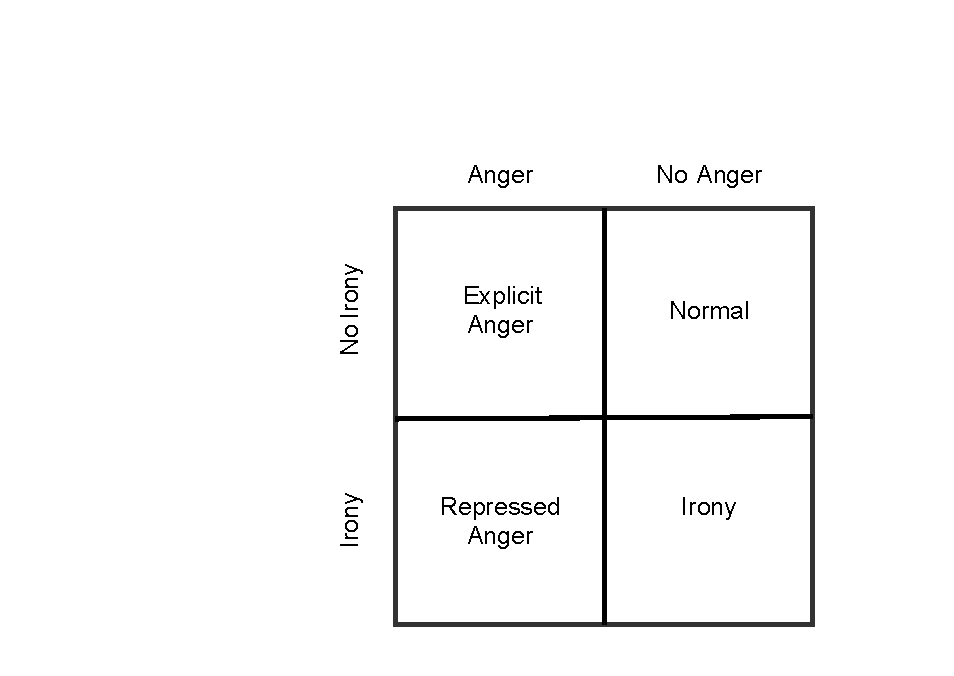
\includegraphics[width=0.6\textwidth]{figures/merge_matrix}
  \caption{Classification prediction output's merge matrix.}
  \label{fig:merge_matrix}
\end{figure}

\iffalse

EMOTEX \& SocialCom: search for tweets with Emotion hashtags from Circumplex model and WordNet Synsets.

[image of EMOTEX system to automatically obtain labeled]

Common Anger Hashtags:
\#angry, \#annoyed, \#annoying, \#bothered, \#frustrate, \#fury, \#furious, \#irritating, \#mad, among many others.

Twitter has made very specific restrictions on redistributing Twitter data, which means that available datasets don't include Tweet text, just a unique identification number.

Retrieve tweet text: python Tweepy API's .get\_status(id) method should do the work.

CrowdFlower public emotion dataset found!

[Data for everyone image]

Crowdflower emotion dataset statistics

40,000 rows of data.
Each row represents a tweet.
13 labels (classes)
Classification: 110 as Anger and 1311 as Hate. Sum: 1421 (3\%)

Conclusions:
Might be a good sample to do a binary classification test:

E.g. 1421 Anger / 1421 Not Anger (others)

Understanding WEKA ARFF file format

Up to now, downloaded datasets were stored as JSON, CSV or Plain Text files. However, WEKA works with a proprietary format file called Attribute-Relation File Format (ARFF).

Completed Task:
Convert downloaded CSV and JSON datasets to ARFF and load them into WEKA to check for possible conversion errors.

(python liac-arff module)

[ARFF file format explanation]

Some simple tests done

Testing WEKA's StringToWordVector to convert ARFF file's tweet messages into more machine learning friendly numerical attributes. (Combined with rainbow stopwords, stemmers, n-gram tokenizers)
Reading about how Random Forest algorithm works and use it to make a rough training and cross-validation classification with random selected features. (5 fold cross-validation results 28.49%)
Resample (Splitting original dataset into, training, validation and testing sets)
Weka's Attribute selection to predict best feature subset (wrappers and rankings) without overfitting.

Next week work

As Crowdflower dataset is composed of 40,000 instances, the resulting matrix from executing WEKA's StringToWordVector tool generates over sparse 10,000 features/attributes without filtering.
Classification of a such a big dataset using SVM or such algorithms takes over 2 hours in generating just the model (on a macbook pro laptop).
Therefore previously proposed 2,841 instances (1421 Anger / 1421 Not Anger) dataset is going to be built in order to be able to test those algorithms in reasonable time.

At the same time while testing new algorithms, information about how they work is going to be read, to understand if the obtained result are the expected.

Continue investigating WEKA and the useful tools it provides for text classification.

Crowdflower emotion dataset is unbalanced

Binary Classification Dataset Generation

Review  Anger and Hate classes and analyse the viability of merging them into a single class.
Checked both classes’ messages, they contain similar information. Therefore the merge is feasible.
Transform the leftover classes into “no anger” class to perform binary classification.
To solve the unbalanced dataset problem there 2 possibilities were studied: 
Use Stratified K-Folds. 
Undersampling the dataset to a more suitable class appearance ratio. (Random permutation of [No. angry tweets] without replacement)
Merge both classes randomly.
Text preprocessing (remove URLs, user mentions, etc.)

Last review’s result:
40,000 instances.
Word2vector, 1-3 n-grams\cite{cavnar1994n} (\~7000 attrs.)
Multi-class classification.
Random Forest (5 CV): 28.49%
This review’s results:
2,866 instances.
Word2vector 1-3 n-grams (\~5000 attrs.)
Binary classification.
Random Forest (10 CV): 63.89%
SVM\\SMO (10 CV): 65.42%
K-NN\\IBK (10 CV): 55.76%
NN (10 CV): Too long (cancelled)

[binary anger dataset distribution image]

Read literature about Convolutional Neural Networks for NLT\cite{cnnDennyBritz}

Use case of CNN for Computer Vision and its translation into NLP.
What is Convolution.
What are Convolutional Neural Networks.
Application into NLP.
CNN Hyperparameters:
Narrow/wide convolution.
Stride size.
Pooling layers.
Channels.

[Remainder] Up to know all the experiments have been done with WEKA’s GUI client and its automatic WordToVector tool.
Now a test using gensim (python word2vec module) has been done for the crowdflower multilabel dataset.
For the trained Word2Vec model, the GoogleNews-Vector(300)\cite{googleWord2Vec} has been used.

publicly available in: \href{https://drive.google.com/file/d/0B7XkCwpI5KDYNlNUTTlSS21pQmM/edit?usp=sharing}{GoogleNews-vectors-negative300.bin.gz}.
Output: 40,000 instances of arrays 31 elements (length of largest sentence for dataset) of 300 features. \~1.27Gb (Untabbed)
Spent time on research how to optimize serialization.
JSON default module Avg. time: \~ 16 mins.
UJSON module Avg. time: < 2 mins.

Expanding the dataset

Found another dataset (Wenbo Wang) that contains labels and tweet id.
Created a Twitter Application to have access to Twitter’s API.
Created a Python module that download tweets based on an id and save all the relevant data into a CSV. (Haven’t tested serialization yet, still downloading.)
This module can be expanded to become a streamer that download tweets based on emotion related hashtags, and get automatic labeled dataset as EMOTEX and SocialCom suggests.

Future Work: Create a CNN

Make a first test for a Deep Learning technique on the ksl-xe5 server.
Since the server does not have graphic cards to speed up the process, I will try to establish connection with my Home server in Spain and replicate the same environment and analyze if there is any performance improvement compared to CPU only computation.
Continue rating the chapter about how traditional classification algorithms work.

Some authors define sarcasm as a sub-set of irony.

Tweet downloader: Wang Dataset

Successfully tested programed module to download Wang dataset. Download tweets into CSV with the following information:
tweet-id, label, author, text-content
However, since dataset is formed with tweets collected from 2011, some of the are unavailable. E.g. From the test.txt, which originally contains 250,000 tweets only 65,324 has been able to be downloaded. (Took 30 hours to download)

TODO: Implement a logger to check if the tweet could not be downloaded due to unavailability or a network failure, for a download retrial.

Started implementing the CNN

Started implementing the Convolution Neural Network (CNN) by using Keras\cite{keras} python module for Deep Learning.
Just need to make some adaptations to the way it parses the word2vec values to be able to test it.
I also investigate how to make full use of the dual graphic card setup of my home server. According to literature I have read there are two techniques to distribute the workflow:
Data parallelization
Model parallelization
The technologies used are based on Message Passing Interface (MPI) architecture. Apparently is not a simple task and the speed up rounds x1.3~x1.6 (last percentage being very unlikely)

Work for next week

Implement the tweet downloader logger to understand why downloads fail, and try to re-download them if network failure.
Finish implementing the CNN.
Do a single GPU test with home server and measure required time to perform the classification.

Tweet downloader

Implemented a basic logger that stores in real time the tweet\_id, error\_code and message on a file. With this simple logger I found these possible errors:
Error 34: Sorry, that page does not exist.
Error 63: User has been suspended.
Error 88: Rate limit exceeded.
Error 114: No status found with that ID.
Error 179: Sorry, you are not authorized to see this status.
Error 500: Internal Server Error.

Error handling (1)

For the previously presented error list there are only two errors that can be handled:
Error 88: Rate limit exceeded.
Error 500: Internal Server Error.
Twitter API enables to download tweets for an interval of 15 minutes, after that it stops providing data for a server request cold down. To solve this error, I make the tweet downloader to wait until the server sends a download acknowledge to resume the download process and avoid getting tweets lost during the cold down interval.

Error handling (2) and logger optimization

Since the Internal Server Error can happen randomly and its duration of the error is unpredictable, the error is recorded for posterior tweet redownload.
As real time loading involves serialization of small chunks of information multiple time, and the error code and message gets repeated it become inefficient and slow down the tweet download. The solution proposed consists on producing a dictionary in RAM and save it into a JSON file with the following structure after the download finishes:

$...
‘code-error (key)’: {
‘tweets’: [
	tweet\_id,
	tweet\_id
	...
]
‘message’: message text.
},
‘No-code-error-message’: {
	‘tweets’: [
	tweet\_id
]
}
...$

Measuring performance

First downloading test consist on downloading tweets from labeled tweet id list. Originally it contained 250,000 tweets. The system was able to download 65,324 tweet text in 30 hours.
After handling the server cold down error the system was able to download 153,387 tweets in 69 hours.
The system maintained almost the same performance after adding the having added the error logger comparing the time spent with the amount of tweets downloaded.

Deep Learning

First basic Deep Learning test implemented using Convolutional Neural Networks (CNN) on Crowdflower multilabel dataset (Keras over TensorFlow). From 40,000 tweets 70\% has been used for training and the remaining 30\% for validation. Has is the first test, 3-grams, 4-grams and 5-grams have been used for the training over the 300 attribute word2vec. Every convolution generates a set of features, but they are discarded for now.
This week I have been able to test on ksl-xe5 server. The results obtained on the training validation accuracy disappointing for 13 label classification, about 26.33\%. It spent 4 hours 30 mins for the training task for 40,000 tweets.

Model characteristics:
Model size: 300
Number of filters: 200
Batch size: 50
Number of epochs: 1000
Evaluation period: 12

Work for the next week

Run the CNN test on home server and try to run on spain university for speed up checking.
Spent some time investigating test preprocessing such as English contraction expansion and misspelled words correction.
Investigate how to improve accuracy in classical and deep learning technique by exploiting features.

Last notes

I have contacted the vice-dean of University of Deusto and ask about how much time I can spend in NUT for the research. Their answer is that I can stay as much time needed, following NUT’s evaluation schedule. 
Meaning that if NUT accept it I could extend my stay in Japan for research as much I NUT allows me.

Deep Learning CPU only vs GPGPU

Last week I was able to test the implemented Convolutional Neural Network on Crowdflower multilabel dataset, based on a TensorFlow and Keras modules.
Using a CPU only configuration on ksl-xe5 server it took 4 hours and 30 minutes to complete the training and validation over the 40,000 tweets.
On the home server running the same test on a GPGPU configuration in conjunction with CUDA 8 and CUDA Deep Neural Network (cuDNN) v5\cite{chetlur2014cudnn}, it took 2 hours 9 minutes to perform the same task. Proving that GPGPU can speed up 52.59\% the process.

Model characteristics:
Model size: 300
Number of filters: 200
Batch size: 50
Number of epochs: 1000
Evaluation period: 12

Test processing
Investigated about expanding unambiguous English contractions to process them into word embeddings. After using a dictionary of contractions and being able to expand them I found that NLTK Stopwords would remove them anyways. A future task would be to investigate if negation is a good feature to extract and if so, remove them from the Stopwords list to the able to process them.
I also investigated Oxford’s Common Misspellings and PyEnchant, a python module that uses OpenOffice dictionaries to correct spelling errors. I will implement a test to check if I can correct misspellings and compare corrected words appearance with the pre-trained Word2Vect model.

Feature extraction

This week I’ve been focused investigating about emotional words lexicon and emoticon lexicon. I have download available lexicons from NRC Emotion Lexicon (EmoLex) and used Wikipedia’s and EMOTEX’s list of emoticons to create an emoticon lexicon. I have used Regular Expressions (regex) to find emoticons on tweets, before the punctuation removal.
The next step would be storing them into the word embeddings to make use of them on CNN, and as a feature for classical classificators.

Future work

During the training phase on the CNN the weights are now static, therefore I will investigate how to make this weights variable.
CNN only work with word embeddings, and do not support the use of other features as with classical classifiers. Due to this I will implement a SVM classifier and use the emoticons, appearance of emotion words, and other features apart from word embeddings.

Spelling check (1)

Last week I talked about a python module called Pyenchant, which provides a function suggest(word) returning an ordered list with the possible corrected words. However it’s accuracy is not very high. Therefore I researched new approaches and found an basic idea proposed from Peter Norvig\cite{PeterNorvigSpell}, Director of Research at Google Inc. He explained that Google search engine uses probability theory to choose the most likely spelling correction for a word (argmax).
argmaxc ∈ candidates P(c) P(w|c)
C ∈ candidates: Candidates model.
P(c): Language model.
P(w|c): Error model.

Spelling check (2)

Candidate model is limited to words with up to 2 editions, correcting splits, deletes, transposes, replaces and insertion errors.
The language model estimates the probability of a words by counting the number of appearance. The tests runs on a dictionary that uses Project Gutenberg’s free eBooks, Wiktionary most frequents words\cite{WiktionaryFL} and \acrfull{bnc} \cite{bncFLAdamK} (Model side ~6Mb.)
The error models prioritizes the original word if it is known, the the list of words known with one modification, followed by the list of words known with two modifications and finally the original word if it is unknown.

Spell checker result using the Big.txt Language Model that Norving Provides.
51\% of 270 correct (35\% unknown) at 37 words per second
53\% of 400 correct (32\% unknown) at 35 words per second

Using the Language Model I generated.
75\% of 270 correct (5\% unknown) at 64 words per second 
69\% of 400 correct (7\% unknown) at 63 words per second

Making some tests

I tested spell correction with the crowdflower dataset. Checking the word that were not numerical. Whenever the spell checker modified a word I printed into the screen so I could do a manual comparison.
I found that the accuracy was better than the enchant module but it continue failing in some cases and all the slang that people uses on the internet was missing in the model, therefore those kind of words were being replaced by a totally unrelated words.
The next step I made was investigating about english slang used on twitter and improving the model accuracy.

Improving the model and twitter slangs (1)

Since the model does not contemplate slang terms found on tweets I have searched for a dictionary of slang with their meaning, so that it can be replaced from the original text during the preprocessing.
To improve the model first I searched for some n-gram database. Google has a huge that includes 5-grams (~22Gb), However the access to this resource costs 150 USD for non-members\cite{LDCGoogle5-gram}. Therefore, I downloaded all the English Ebooks from Project Gutenberg as for 2014 from Kiwix harvester\cite{kiwix} (~42Gb) publicly available from \url{http://download.kiwix.org/zim/gutenberg/gutenberg_en_all_10_2014.zim}. After solving encoding errors in some file names I start the eBook preprocessing.

Improving the model and twitter slangs (2)

Since all the eBooks are stored as \acrfull{html} document, I removed all the \acrshort{html} tags from the texts, to improve later on model generation performance, it took 1 hour 38 mins to remove all the \acrshort{html} tags.
I programmed a python module that take the requested model size as argument and concatenates as many eBooks until reaching requested size.
The Spell checker now read the model generated from this book concatenation, but next step would be to generate a word counter and store this document as a model instead to improve even more spell checker performance.

Spell checking model redesigned

On the previous I stated that I programmed a python module that removes the \acrshort{html} tags from Project Gutenberg's eBooks and concatenates it into a single document to. Last week I redesigned this module.
Now, the program search for word frequency files from eBooks and generates a single dictionary with the word occurrences from each document.
If the word frequency file does not exists for a certain eBook it process the document by checking if it contains \acrshort{html} tags and if so remove them, overwriting the original file in the process.
Calculates the word frequency for that eBook and saves it into a file while at the same time updating the global dictionary that contains the words for all documents.
This way if the program has to run a second time it does not have to start all the process from the beginning.

Adding twitter scope words to spelling model

Merge Datasets

Programmed a python module that receives as input a list of dataset paths and a sentiment target label “mapper” file. 
With this information perform a dataset concatenation, and transforms labels as the mapper file states and filter tweets that contains non-english characters, typical from Spanish, Portuguese and French, found on Wang dataset.
It can also transform the dataset labels into “anger” and “no\_anger” classes, used for binary classification.

Generalize Python Modules

Since all the programmed modules inputs and outputs were hardcoded, I spent time on making them variable arguments introduced on console line.
This would ease me testing the programmed modules with different datasets, such as word2vec transformation and Convolutional Neural Network (CNN) classification.

Convolutional Neural Networks Binary Classification Test

My last test with CNN I used Crowdflower’s dataset, consisting in 40,000 tweets with 13 sentiment target labels. The dataset was divided in 70\% training 30\% validation. After training the validation accuracy the system scored was 26.33\%. Then I made a second test using the spelling checker on the word2vec process. If a word could be found in the model it would check it’s spelling and replaced with the suggested word correction. The accuracy the system scored after apply this simple modification was 27\%. For my last test I decided to change the dataset. I merged Crowdflower’s dataset and Wang’s test.csv and transform it into a binary class label dataset, representing 33,752 “anger” and 33,752 “no\_anger” tweets. Again, using the spellchecker on word2vec process I run the CNN classification and obtained a 99.73\% validation accuracy.

Convolutional Neural Networks Binary Classification Test

Since the result were so good I thought I did something wrong, and check that the merged dataset was formed correctly without repeated data. But apparently it is OK. Therefore, since I didn’t have 21,000 tweets for creating proper size test dataset and I did not have time to retrain the model again and re-split the dataset, I took my remaining small “train” dataset I had from Wang dataset, containing 282 tweets. I made a binary dataset with that and used as test data. By using the model weight I got from the training and validation process I test the new unclassified 282 binary labeled tweets. The system achieved a 100\% accuracy on the testing phase over that small dataset.

Future work

Add slang dictionaries and test crowdflower dataset to check if performance improves.
Continue emoticon and emotion words feature extraction.
Continue implementing SVM classifier.
Split the dataset into 70\% train 15\% validation 15\% test and re-run the CNN module and recheck the results over binary classification.
Calculate Precision, Recall and F1-score.

Last week I made the first CNN accuracy evaluation that achieved 99.73\%, but the test size was 282 tweets, compared to 21,200 tweets used in the evaluation, which was not enough.
Due to that, I made modifications into the module that transform the dataset into word embeddings to be able to split the dataset into 70\% training, 15\% validation and 15\% testing.
Right away, I made another CNN training, and validation and testing, and confirmed that the accuracy was really of 99.73\%

CNN: Speed up training phase

During last test I made I realise that most of the time of the training phase, the model was not learning anything new, after the maximum validation accuracy was reached. Therefore I spent time or investigating how to stop the training phase when no more gain was scored. I found the following relevant classes:
EarlyStopping: Stop training when a monitored quantity has stopped improving (‘val\_loss’)
ModelCheckpoint: Save the model after every epoch. (Save only best model)
Spent time comparison:
Before modifications: \~9 hours 30 mins.
After modifications: \~10 mins. (Stopped after 22 Epoch)

Confusion Matrix and Scikit evaluation

To evaluate that what I was doing was right I created a confusion matrix with the method Keras library provided, plus what I researched about how to make diagrams with matplotlib’s pyplot. The result was this:

[image of confusion matrix]

Scikit evaluation\cite{scikit-learn}

Since I cannot the data I got from Keras I used scikit to check if the predictions CNN make are correct. I for the confusion matrix I was also able to calculate the following evaluation metrics:
Accuracy: 0.9974323524
Recall (macro): 0.9974325863
Precision (macro): 0.997434915
F1-score (macro): 0.9974323499

Cuda installation on arrived server (1)

I tried to follow my own installation guide I made several weeks ago and try to install Fedora 24. However, the combination of Skylake and Pascal architecture has made the more difficult.
Skylake requires Linux kernel 4.5.5 to work.
Fedora 24’s open-source video drivers don’t work with Pascal architecture, so after grub menu in the OS installation process the screen becomes black.
Therefore I tried to Install Fedora 25, that run’s wayland by default instead of X server. Nevertheless, I found that Nvidia does not support the kernel source that packs Fedora 25 and makes difficult its installation.

Cuda installation on arrived server (2)

So I decided that I would keep to my original idea to install Fedora 24. To do so I read that first I had to disconnect the Nvidia GPU out of the PCI slot. After almost 1 hour trying to pull out the GPU out of the board (It was stuck on the PCI port) I was able to run the Fedora 24 live USB and install it.
This week, I will check if there is any problem with kernel version and Nvidia. But if I find any problem that makes difficult the cuda toolkit installation, my last attempt will be to install Ubuntu 16.04

Future work

Add slang dictionaries and test crowdflower dataset to check if performance improves.
Continue emoticon and emotion words feature extraction.
Continue implementing SVM classifier.
Fix CNN accuracy lost after serializing model.
Install all CUDA Server’s dependencies.
Search for an irony dataset to make test with CNN.

Download Irony and Sarcasm tweets
Previously I read some literature about Irony and Sarcasm. Some authors define sarcasm as part of Irony. Others state that is a figurative language completely different. For my research due to the reduced amount of data I have found so far, I will deal with these term as if they were equal.
With the tweet-downloader module I have been able to download tweet that contain the \#irony, \#ironic or \#sarcasm hashtags in tweets. Up to now the system has downloaded 18,398 tweets, which I still need to preprocess and filter.

Preprocess Irony Dataset
I used a Google Sheets extension called Twitter Archiver that remotely downloads tweets and saves it into a Google Sheets document.
As I said on last group meeting, I was downloading English Tweets that contained \#irony, \#ironic and \#sarcasm hashtags.
I have managed to download a total of 34.000 tweets (still downloading)
I need to remove useless columns from the CSV, rename columns names to be able to use with my python modules, remove duplicate tweets documents (Retweets) and remove these 3 hashtags from the text.
I created a python module that performed all the tasks from last point.

Perform Irony Dataset CNN Test

Dataset characteristics:
Instances: 56,264 tweets.
Balanced 50\% irony (28,132)
2 target labels, (binary)
Split: 70\% train. 30\% val.
Val. Acc: 91.88\% (w/u spell)
Val. Acc: 91.86\% (w. spell. chckr)

Recall (macro): 0.9188087708
Precision (macro): 0.9188862312
F1 (macro): 0.9188298366

Note: With the spell checker the CNN losses accuracy for this dataset. To implement a more complex spelling checker would be needed, + other techniques (stemming, lemmatization, synonyms).

Model characteristics:
Model size: 300
Number of filters: 200
Batch size: 50
Number of epochs: 1000
Evaluation period: 12

Found a bug in Anger Dataset

Anger dataset is generated by merging the Crowdflower dataset and Wang test dataset.
When I created the dataset I checked that Crowdflower tweets didn’t contain hashtags such as \#anger, \#rage, etc. However I forgot to check that on the Wang dataset, which  DO contain them. I modified the dataset merger module to find those hashtags and remove them from the tweet content. After doing it a performed again the CNN to recheck the results:

Dataset characteristics:
Instances: 67,504* tweets.
2 target labels
Acc: 99.64\~99.74\%

Dataset characteristics:
Instances: 70,108 tweets.
2 target labels
Acc: 95.92\% (w/o spell)
Acc: 96.15\% (w. spell chkr)

Note: Used less tweets on first test because I removed all the duplicated tweets. Now the merger maintains the first instance. (fixed)

Future work
Investigate how to combine both anger and irony classificators and do a final test with that classifier. (Ensemble Learning?)

Continue implementing SVM classifier.
Add slang dictionaries and test crowdflower dataset to check if performance improves.
Continue emoticon and emotion words feature extraction.
Fix CNN accuracy lost after serializing model.

CNN module
After training and validating the model, serializing it and loading the weights for posterior executions would produce a considerable accuracy lost on the classifier (\~51\%). This issue has been already fixed. The possibility of storing the models and make the weights reusable enables to program successive module that uses all the pre-trained classifiers to combine their results to detect repressed anger tweets.
Fixed a bug with the Confusion Matrix Drawer, not rendering the normalized version of the matrix properly.
Standardized the output to easily be able to use the results into the next module that combines all classifiers.

Read literature (Model combination)

Since I have two classifiers that can detect anger and irony independently, I have read some papers about the techniques used to combine the classifiers to be able to use the to detect repressed anger. First I thought about Ensembled Learning’s Divide and Conquer technique, with a voting combination rule. However after Asking to Yukawa sensei he proposed to build a 2x2 matrix to classify the output as following (right):

[Image of divide and conquer technique]

[image of 2x2 combination matrix]

I started programming the module that combines the classifiers. It already loads the classifiers. However I have to preprocess the dataset on a different way to proceed with the prediction and combination.

[image of the merge to word2vec process]

Note: Combined test dataset fragment is used in the final step’s prediction phase.

Question:
Can the binary anger and binary irony datasets’ no\_irony and no\_anger have tweets in common?

Finished dataset preparation

[image of the merge to word2vec process]

Implemented the dataset preparation system that I presented last week.
Around unique 220,000 gathered after merging all datasets.
Re-splitted dataset into anger and irony binary dataset with no common tweets with 67,746 and 56,264 tweets respectively. (removing key hashtags)
Resulting dataset were divided into 73\% train, 18\% validation and 9\% test.
Anger and irony’s tests dataset were merged generating a the final prediction file of 11,060 tweets.

Pre-training the classifiers and prediction

Resulting train and evaluation word embeddings are used for classification learning process, generating model structure and model weights files.
Test word embeddings are used to generate an approximate performance record sample.
With the model structure and weights and the merged test dataset, a CSV with the prediction result is generated.
A evaluation method for this last step is still missing.

[image from word2vec to final prediction process]

Searching for evaluation method

[image of excel with the classification labels, half of the prediction can be done]

To validate the prediction, Yukawa sensei suggested to perform a manual classification of the dataset

Dataset manual classification

As doing a single classification is not reliable, I created a program with google app script that automatically creates google forms based on the dataset data.

I will send to some friends to help me with this task, in order to improve the reliability of the manual classification.

[various images of google tech, code, forms and results]

Doubt: Using hashtags or remove them

Example 1:

I \#hate when I have to meet my neighbors in the morning. (in sentence natural usage)

Example 2:

I had to explain my parents once again how to use the refrigerator due to Alzheimer \#sad 
(out sentence usage for classification)

The second usage case alters the results of the classification. But since I cannot differentiate between all the tweets of the dataset, I think that I should remove all the dataset, (even if some of the sentences lose meaning) because the second case (majority) is faking the result of the learning process. 

Re-run the learning process (no hashtags)

After re-running the learning process of both classifiers and check their individual accuracy score it when down to 78\% and 84\% for anger and irony respectively

\fi